\section{بخش دوم: تحلیل نویز (\lr{Noise Analysis})}

\begin{stepbox}
\field{تزریق نویز گوسی (\lr{Gaussian Noise})}{
در این بخش، نویز گوسی با میانگین صفر ($n \sim \mathcal{N}(0, \sigma^2)$) و مقادیر انحراف معیار مختلف ($\sigma \in \{10, 25, 50\}$) به صورت دست‌ساز تولید شده و به تصویر اضافه می‌گردد. سپس تاثیر تغییر انحراف معیار بر خصوصیات بصری و آماری تصویر مورد ارزیابی قرار می‌گیرد.
}
\end{stepbox}

\begin{codebox}[تولید و اعمال نویز گوسی به تصویر]
\begin{lstlisting}[language=Python]
scales = [10, 25, 50]
fig, axes = plt.subplots(3, 2, figsize=(12, 12))

for i, scale in enumerate(scales):
    # تولید نویز گوسی بر اساس انحراف معیار مشخص
    noise = np.random.normal(loc=0.0, scale=scale, size=sample_image.shape)
    noisy_sample = sample_image + noise
    
    # برش مقادیر خارج از بازه استاندارد تصویر [0, 255]
    noisy_sample_clipped = np.clip(noisy_sample, 0, 255).astype(np.uint8)
    
    axes[i, 0].imshow(noisy_sample_clipped)
    axes[i, 1].hist(noisy_sample_clipped.flatten(), bins=50, color='blue', alpha=0.7)
\end{lstlisting}
\end{codebox}

\begin{figure}[htbp]
    \centering
    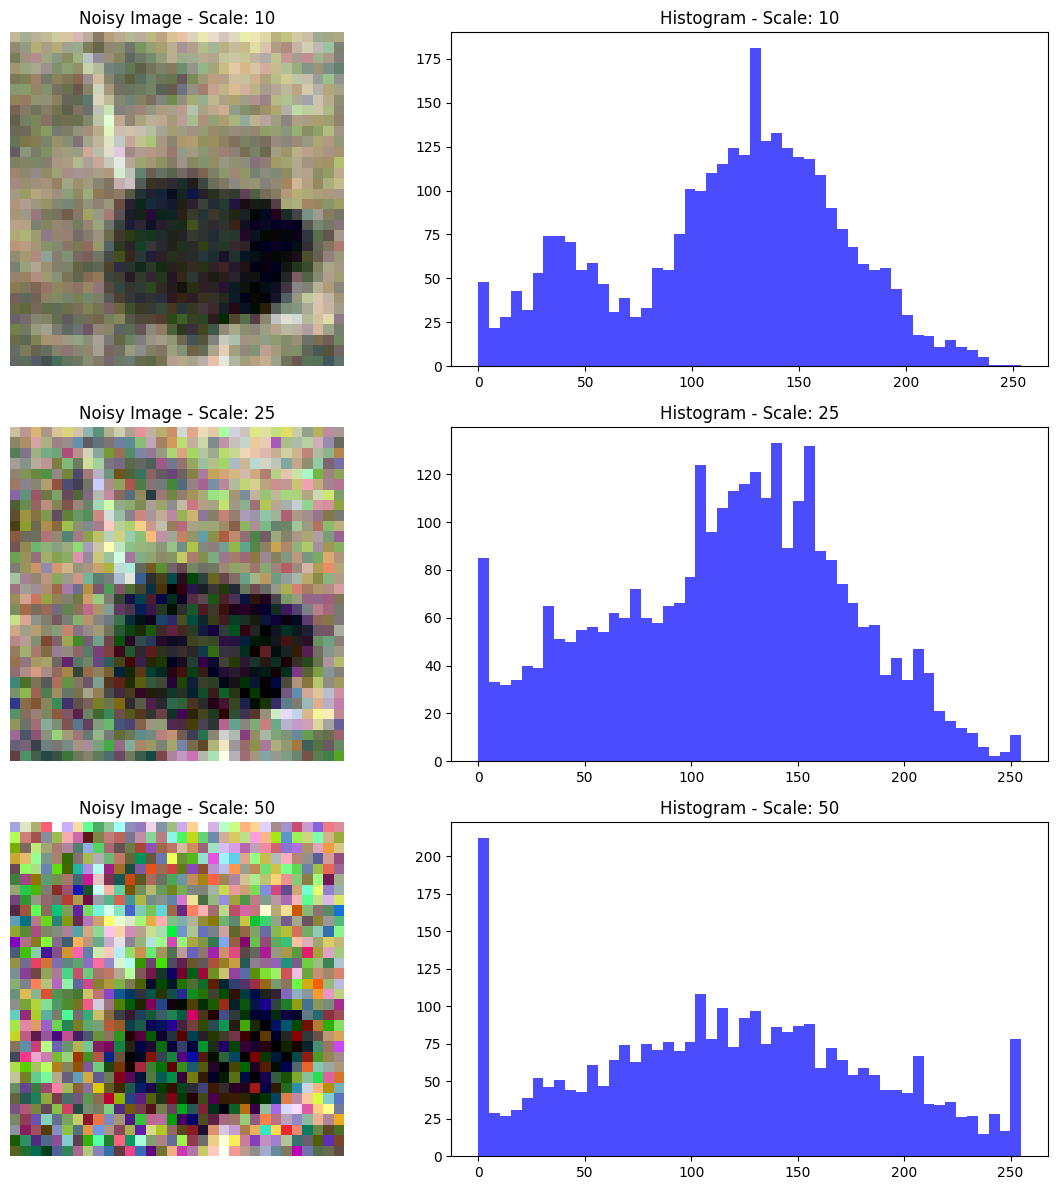
\includegraphics[width=0.88\textwidth]{images/img_noise_comparison.png}
    \caption{بررسی اثر افزایش انحراف معیار نویز ($\sigma$) بر کیفیت تصویر و هیستوگرام مربوطه}
    \label{fig:noise_grid}
\end{figure}

\begin{stepbox}
\field{تحلیل آماری و رفتار داده‌ها زیر نویز}{
\textbf{۱. تغییرات بصری (\lr{Visual Changes}):} \\
با افزایش $\sigma$، میزان نوسانات تصادفی شدت روشنایی افزایش یافته و ساختارهای ظریف و لبه‌های تصویر زیر پوشش نویز یا حالت برفکی (\lr{Grainy Artifacts}) ناپدید می‌شوند.

\textbf{۲. میانگین (\lr{Mean}):} \\
از آنجا که نویز افزوده شده دارای میانگین صفر ($\mu = 0$) است، مقدار انتظاری نویز صفر بوده و میانگین کل شدت روشنایی تصویر ($\mathbb{E}[X + N] = \mathbb{E}[X] + \mathbb{E}[N] = \mathbb{E}[X]$) تقریباً ثابت باقی می‌ماند (به جز تغییرات ناچیز حاصل از عملیات برش یا \lr{Clipping}).

\textbf{۳. واریانس (\lr{Variance}):} \\
با توجه به استقلال نویز از تصویر، واریانس تصویر نویزی برابر با مجموع واریانس تصویر اصلی و واریانس نویز است ($\text{Var}(X + N) = \text{Var}(X) + \sigma^2$). بنابراین با افزایش $\sigma$، واریانس تصویر به صورت خطی رشد می‌کند.

\textbf{۴. هیستوگرام (\lr{Histogram}):} \\
با افزایش نویز، قله‌های تیز هیستوگرام پهن‌تر شده و شکل توزیع کلی به سمت منحنی زنگوله‌ای (\lr{Bell Curve}) مربوط به توزیع نرمال سوق پیدا می‌کند؛ به‌طوری‌که در $\sigma = 50$ توزیع نویز بر توزیع اصلی تصویر غلبه می‌کند.
}
\end{stepbox}